\enlargethispage{2cm} % zvětší tiskové zrcadlo dané stránky

\vspace*{-2cm}

\thispagestyle{empty} %%%%%%%%%%%%%%%%% titulní strana nemá číslování
%
\setcounter{page}{0} % nastaví číslo této stránky na 0


\begin{center}
	
\Large

Jaroslav Páral 

Jakub Streit 

Rudolf Hlaváček

a další 

\vskip 1cm



\Huge \bf 

ROBOTICKÝ MANUÁL 

\large

aneb

\LARGE

Co se hodí vědět při stavbě 

a programování hobby robotů


\vskip 1cm

\Large

%\begin{figure}[h]
%    \begin{center}
%          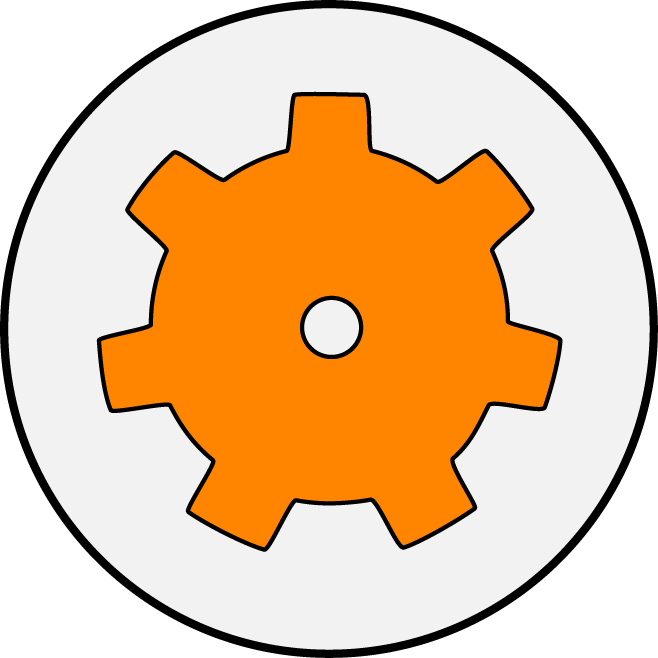
\includegraphics[width=0.3\textwidth]{soubory/robotarna_logo_edit_kolecko.png}
%        
\includegraphics[width=1\textwidth]{soubory/robotarna_logo_edit.png}
%    \end{center}
%\end{figure}	


{\tt www.robotarna.cz}

\vskip 0.5cm

{\tt www.sokolska.cz}

\vskip 0.5cm

{\tt www.robotikabrno.cz}


\vskip 1.2cm


za kolektiv autorů

Miroslav Burda

editor 

\vskip .7cm

{\tt dokumentace@robotikabrno.cz}

\vskip 1cm  
	
verze 1.0 

{\tt \today{ }\DTMcurrenttime}

{\tt \large PDF:\href{https://doc.robotikabrno.cz/RoboticsManual.pdf}{doc.robotikabrno.cz/RoboticsManual.pdf}}

{\tt \large Online verze:\href{https://doc.robotikabrno.cz/}{doc.robotikabrno.cz}}
	
\end{center}
